
\chapter{SELKS}
\label{chap:selks}

\definition{SELKS}{SELKS is a free and open source Debian (with LXDE X-window manager) based IDS/IPS platform released under GPLv3 from Stamus Networks (https://www.stamus-networks.com/).\cite{stamusnetworks:_selks}~\\

The SELKS ISO is both Live and Installable ISO in one. Once installed it is ready to use out of the box solution. ~\\

SELKS is comprised of the following major components:
\begin{itemize}[itemsep=0pt]
\item[\textbf{S}] Suricata IDPS - http://suricata-ids.org/
\item[\textbf{E}] Elasticsearch - http://www.elasticsearch.org/overview/
\item[\textbf{L}] Logstash - http://www.elasticsearch.org/overview/
\item[\textbf{K}] Kibana - http://www.elasticsearch.org/overview/
\item[\textbf{S}] Scirius - https://github.com/StamusNetworks/scirius
\end{itemize}
}

So SELKS is an OS which contain the Suricata IDS. It also contain Elasticsearch to analyze alerts, Logstash to
analyze log, Kibana to have overview of alerts, and Scirius to add rules.

You can see on figure \ref{fig:kibana}, an example of the interface of kibana which give an overview of the alerts.
This image was extract from the Twitter of Stamus Networks.



\begin{figure}
  \centering
  
\includegraphics[width=\textwidth]{selks_desktop}
  \caption{screenshot of SELKS desktop}
  \label{fig:selks}
\end{figure}

\begin{figure}[h]
  \centering
  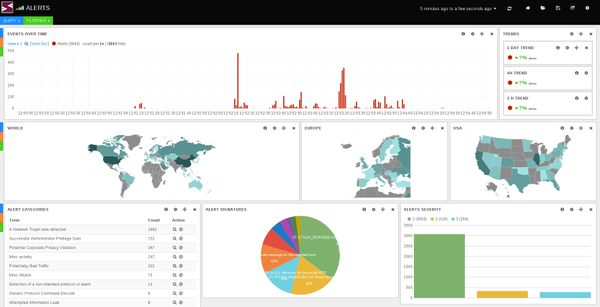
\includegraphics[width=\textwidth]{kibana}
  \caption{Kibana interface}
  \label{fig:kibana}
\end{figure}


%%% Local Variables:
%%% mode: latex
%%% TeX-master: "../rapport_de_base"
%%% End:
